\documentclass[12pt]{IEEEtran}
\usepackage{hyperref}
\usepackage{listings}
\usepackage{color}
\usepackage{xcolor}
\usepackage{graphicx}

\definecolor{dkgreen}{rgb}{0,0.6,0}
\definecolor{gray}{rgb}{0.5,0.5,0.5}
\definecolor{mauve}{rgb}{0.58,0,0.82}

\lstset{frame=tb,
  language=C++,
  aboveskip=3mm,
  belowskip=3mm,
  showstringspaces=false,
  columns=flexible,
  basicstyle={\small\ttfamily},
  numbers=none,
  numberstyle=\tiny\color{gray},
  keywordstyle=\color{blue},
  commentstyle=\color{dkgreen},
  stringstyle=\color{mauve},
  breaklines=true,
  breakatwhitespace=true,
  tabsize=3
}


\author{Clay Buxton}
\title{%
Chocolate Chip \\
\large A well-documented, informative, and simple CHIP-8 Emulator}

\date{\today}
\begin{document}
\maketitle

\textbf{Repository} \href{https://github.com/clbx/ChocolateChip}{https://github.com/clbx/ChocolateChip}

\section{Abstract}
CHIP-8 is an interpreted machine language built in the 1970's for 8-bit
micro computers. Today the only way to run a CHIP-8 program is through emulation.
The goal of this project was to accurately emulate the CHIP-8 architecture. 
The CHIP-8 emulator is generally regarded as a simple emulation project and a good first step into 
the world of emulation. Chocolate Chip was designed to be easily readable, documented, and informative emulator,
in addition to properly running a long lost architecture.

\section{Introduction}
ChocolateChip is written in C++ and primarily focused on giving the user the entire picture of what is happening inside
the machine opposed to just simply emulating it. The CHIP-8 architecture is much simpler to emulate than many other architectures due
to it's small amount of opcodes and being contained in one process. Chocolate Chip has a status screen that displays the last few opcodes 
executed with a line reading out what they do and their effect on the system, the status of the registers, the position in memory being pointed to, the keys being pressed, and the status of the stack.
This is all throughly documented as well.

\section{Installation}

\textbf{Requirements}
\begin{itemize}
    \item \href{https://www.sfml-dev.org}{SFML} For graphics
    \item \href{http://fmtlib.net/latest/index.html}{fmt} For properly formatting the logger
    \item \href {https://github.com/google/googletest}{gTest} if you want to run the unit tests
\end{itemize}

\textbf{Installation}


\begin{itemize}
    \item Install the dependancies for your system
    \item Clone the repository\\ 
    \colorbox{gray!30}{git clone https://github.com/clbx/ChocolateChip}
    \item Run \colorbox{gray!30}{make}
\end{itemize}



\section{Methodology}
Chocolate Chip is divided into 3 classes, the Emulator, the Application and the Logger.
The application portion displays the graphics and receives input from the user. The emulator takes an instruction from the program file, and the logger records current status for the user.
\\
The Application portion shows a window of the currently running program and process user input (the 0-9 and A-F "keys")
\begin{figure}[h]
    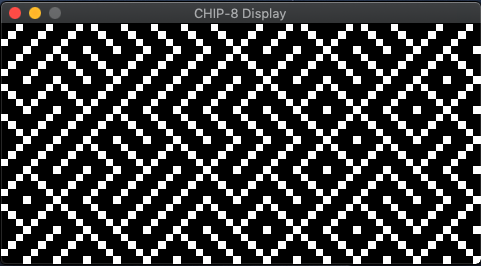
\includegraphics[width=\linewidth]{application.png}
    \caption{The application window shown running the maze generator}
\end{figure}

This is done using the SFML graphics library, on every tick of the emulator the application redraws the screen based on the status of a pixel buffer.
However this will eventually be improved in the future since only 2 opcodes actually affect graphics and redrawing on every tick is inefficient
\\
\\The emulator takes and processes and instruction. In the CHIP-8 architecture, the code memory is put in the same place as the usable memory, so reading a program consists of
loading a ROM into memory and executing opcodes found at the first memory address and then moving on. The emulator then processes each opcode and moves on to the next instruction
\\
The logger outputs information to the user about the last few executed opcodes and the current status of the registers, address pointer, and program counter
This was a feature I wanted to focus on this project so anyone can see what the emulator is doing at any time. This gives a simple way to peering into what is happening behind the scenes
\begin{figure}[h]
    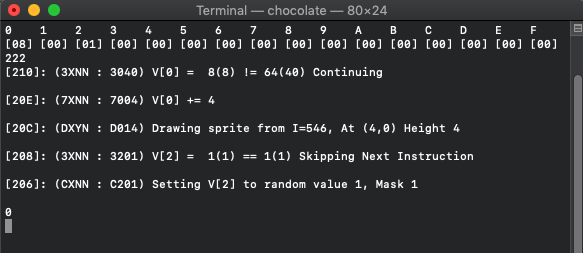
\includegraphics[width=\linewidth]{logger.png}
    \caption{The logger window that shows information about the emulator}
\end{figure}


\section{Results}
As of the final for CS333 all of the opcodes are implemented. Graphics word correctly and many basic ROMs run perfectly.
Options are given to the user to run the emulator in different modes and speeds. The logger is fully functional. However, no unit tests have been written due to a good way of testing them
Many more advanced games are buggy and unplayable, however simpler ROMs that do not rely on graphic collision calculation work flawlessly.

\section{References}
\begin{itemize}
    \item Cowgod's Chip 8 Reference\\ \href{http://devernay.free.fr/hacks/chip8/C8TECH10.HTM}{http://devernay.free.fr/hacks/chip8/C8TECH10.HTM}
    \item Multigesture How to build an emulator\\ \href{http://www.multigesture.net/articles/how-to-write-an-emulator-chip-8-interpreter/}{http://www.multigesture.net/articles/how-to-write-an-emulator-chip-8-interpreter/}
    \item Wikipedia's CHIP-8 Page\\ \href{https://en.wikipedia.org/wiki/CHIP-8}{https://en.wikipedia.org/wiki/CHIP-8}
\end{itemize}


\end{document}
